\section{Markov Chain Monte Carlo}
\subsection{Markov Chain}
In most cases, we assume the samples are independent. However, it is a poor assumption as this may rarely happen in reality. Therefore, we assume the data are dependent and hence we have \textbf{sequential data}. More specifically, we can use \textbf{markov chain} to model the sequential data.
\begin{figure}[H]
    \centering
    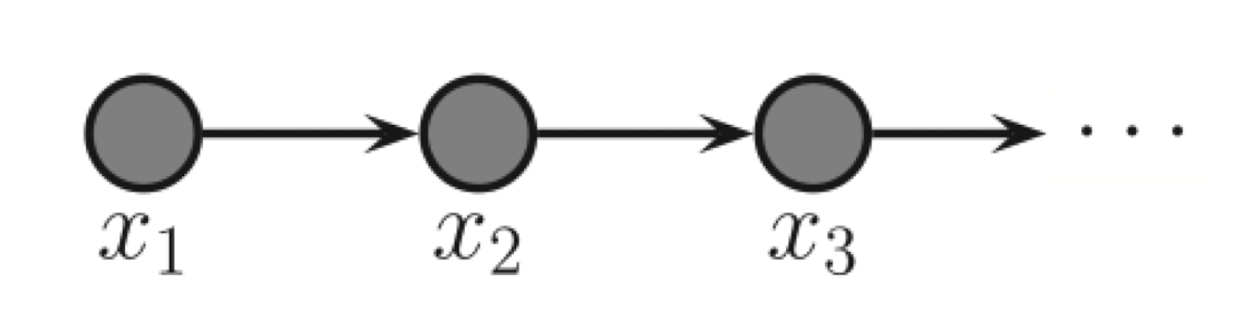
\includegraphics[width = .6\linewidth]{figures/section6/figure_6_1.png}
    \caption{First order Markov Chain}
    \label{fig:f_mc}
\end{figure}
\hyperref[fig:f_mc]{Figure 6.1} shows an example of First order Markov chain.
\begin{align*} 
    p\left(x_t \mid x_{1: t-1}\right)&=p\left(x_t \mid x_{t-1}\right)\\
    &=\prod_{t=1}^T p\left(x_t \mid x_{t-1}\right)
\end{align*}
From the graph, we can see that the first order means each node is conditioned on the previous node. We can therefore generalize to higher order Markov Chains.
\begin{itemize}    \item For second-order Markov Chains:
    $$p\left(x_t \mid x_{1: t-1}\right)=p\left(x_t \mid x_{t-1},x_{t-2}\right)$$
    \item For m-order Markov Chains:
    $$p\left(x_{1: T}\right)=p\left(x_t \mid x_{t-1:t-m}\right)$$
\end{itemize}
We have two further definations:\\
\textbf{Stationary(homongeneous) Markov Chain}: The distribution generating the data does not change over time:
$$p(x_{t+1}=y|x_t=x)=p(x_{t+2}=y|x_{t+1}=x)$$ 
\textbf{Non-stationary Markov Chain}: $p(x_{t+1}=y|x_t=x)$ depends on time $t$.